%Préambule du document :
\documentclass[12pt]{report}
\usepackage[top=2cm,bottom=2cm,left=2cm,right=2cm]{geometry}
\usepackage[utf8]{inputenc}
\usepackage[francais]{babel}
\usepackage{color}
\usepackage{graphicx} 
\usepackage{url}
\usepackage{hyperref}
\usepackage[T1]{fontenc}
\usepackage{float}
\usepackage{array}

\usepackage{listingsutf8} % ne change rien, a virer ?

% pour code source
\usepackage{listings}
\lstset{
	basicstyle=\footnotesize,
	%extendedchars=\true
	%inputencoding=utf8/latin1
	numberstyle=\footnotesize,
	frame=single,
	tabsize=2,
	breaklines=true,
	backgroundcolor=\color{rltgrey},
	keywordstyle=\color[rgb]{0,0,1},
	commentstyle=\color[rgb]{0.133,0.545,0.133},
	stringstyle=\color[rgb]{0.627,0.126,0.941},
}

\definecolor{red1}{RGB}{153,0,0}
\definecolor{rltgrey}{rgb}{0.9,0.9,0.9}
\definecolor{rltblue}{rgb}{0.5,0.7,0.9}
\hypersetup{colorlinks,%
            citecolor=black,%
            filecolor=black,%
            linkcolor=black,%
            urlcolor=red1}


%Page de Garde
\makeatletter
\def\clap#1{\hbox to 0pt{\hss #1\hss}}%
\def\ligne#1{%
\hbox to \hsize{%
\vbox{\centering #1}}}%
\def\haut#1#2#3{%
\hbox to \hsize{%
\rlap{\vtop{\raggedright #1}}%
\hss
\clap{\vtop{\centering #2}}%
\hss
\llap{\vtop{\raggedleft #3}}}}%
\def\bas#1#2#3{%
\hbox to \hsize{%
\rlap{\vbox{\raggedright #1}}%
\hss
\clap{\vbox{\centering #2}}%
\hss
\llap{\vbox{\raggedleft #3}}}}%
\def\maketitle{%
\thispagestyle{empty}\vbox to \vsize{%
\haut{}{\@blurb}{}
\vfill
\vspace{1cm}
\begin{flushleft}
\usefont{OT1}{ptm}{m}{n}
\huge \@title
\end{flushleft}
\par
\hrule height 4pt
\par
\begin{flushright}
\usefont{OT1}{phv}{m}{n}
\Large \@author
\par
\end{flushright}
\vspace{1cm}
\vfill
\vfill
\bas{}{\@location, le \@date}{}
}%
\cleardoublepage
}
\def\date#1{\def\@date{#1}}
\def\author#1{\def\@author{#1}}
\def\title#1{\def\@title{#1}}
\def\location#1{\def\@location{#1}}
\def\blurb#1{\def\@blurb{#1}}
\date{\today}
\author{}
\title{}
\location{Nancy}\blurb{}
\makeatother
\title{\textcolor[RGB]{153,0,0}{Système de fichiers distribué : comparaison de GlusterFS, MooseFS et Ceph avec déploiement sur la grille de calcul Grid’5000.}}
\author{Jean-François Garçia, Florent Lévigne,\\Maxime Douheret, Vincent Claudel.}
\location{Nancy}
\blurb{%
IUT Nancy-Charlemagne Université Nancy 2\\
\textbf{\textcolor[RGB]{153,0,0}{Licence Professionnelle Asrall}}\\[1em]
Tuteur : Maître de Conférences : Lucas Nussbaum\\
}% 


%definition des pages
\makeatletter
\def\thickhrulefill{\leavevmode \leaders
\hrule height 1ex \hfill \kern \z@}
\def\@makechapterhead#1{%
\vspace*{10\p@}%
{\parindent \z@
{\reset@font
\usefont{OT1}{phv}{m}{n}
\LARGE Partie \thechapter\par\nobreak}%
\par\nobreak
\vspace*{30\p@}
\interlinepenalty\@M
\usefont{OT1}{ptm}{b}{n}
{\raggedright \Huge \bfseries #1}%
\par\nobreak
\vskip 20\p@
\hrule height 2pt
\par\nobreak
\vskip 45\p@
}}
\def\@makeschapterhead#1{%
\vspace*{10\p@}%
{\parindent \z@
{\raggedleft \reset@font
\scshape \vphantom{\@chapapp{} \thechapter}
\par\nobreak}%
\par\nobreak
\vspace*{30\p@}
\interlinepenalty\@M
\usefont{OT1}{ptm}{b}{n}
{\raggedright \Huge \bfseries #1}%
\par\nobreak
\par\nobreak
\vskip 45\p@
}} 



%Corps du document :
\begin{document}
	\maketitle
	\tableofcontents

	\chapter{Introduction}
		\section{Contexte}
			Étudiants en licence professionnelle ASRALL (Administration de Systèmes, Réseaux, et Applications à base de Logiciels libres),
			notre formation prévoie une période de deux mois à mis temps pour la réalisation d'un projet tuteuré.

			Le projet que nous avons choisis consiste à comparer diverses solutions de systèmes de fichiers distribués.

		\section{Système de fichiers distribué}
			% Très fortement inspiré de Wikipédia (citer sources en fin de rapport)
			% système de fichier distribué basé sur un fs "normal" ?
			Un système de fichiers (file system en anglais) est une façon de stocker des informations et de les organiser dans des fichiers,
			sur des périphérique comme un disque dur, un CD-ROM, une clé USB, etc.
			Il existe de nombreux systèmes de fichiers (certains ayant des avantages sur d'autres),
			dont entre autre l'ext (Extented FS), le NTFS (New Technology FileSystem), ZFS (Zettabyte FS), FAT (File Allocation Table).
			
			Un système de fichiers distribué est un système de fichiers permettant le partage de données à plusieurs clients
			au travers du réseau.
			Contrairement à un système de fichier local, le client n'a pas accès au système de stockage sous-jacent,
			et interagit avec le système de fichier via un protocole adéquat.

			Un système de fichier distribué est donc utilisé par plusieurs machines en même temps
			(les machines peuvent ainsi avoir accès a des fichiers distants, l'espace de noms est mis en commun).
			Un tel système permet donc de partager des données entre plusieurs client,
			et pour certains de répartir la charge entre plusieurs machines, et de gérer la sécurité des données
			(par réplication)

                        \newpage
		\section{Le Grid'5000}
		Le Grid'5000 est une infrastructure distribuée de neuf sites sur la France, dédié à la recherche,
		sur des systèmes distribuées à grande échelle.

		Les ingénieurs assurant le développement et le support de l'infrastructure jour après jour viennent pour la plupart	de l'INRIA\footnote{Institut National de Recherche en Informatique et en Automatique}.

		Le Grid'5000 est répartit sur onze sites, dont neuf en France.

		\begin{figure}[H]
			\begin{center}
				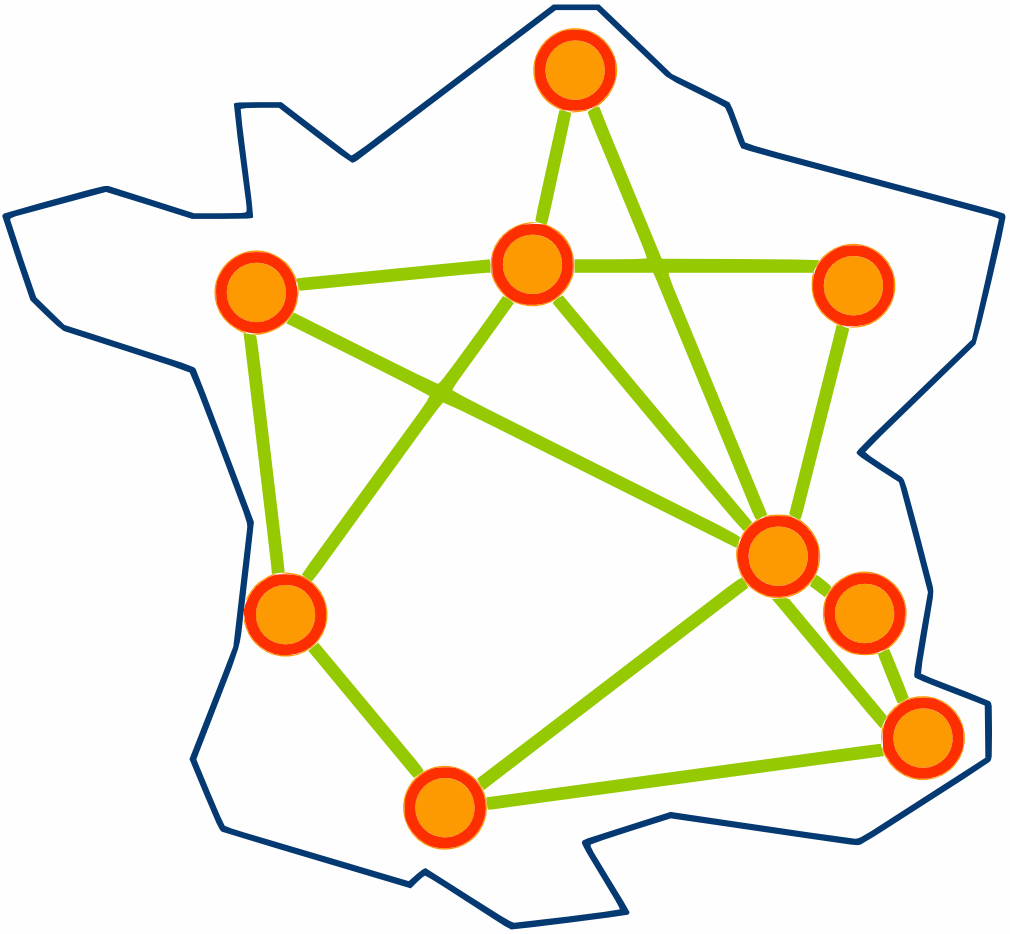
\includegraphics[width=0.4\linewidth]{images/Site_map.png}
				\caption{Les sites français du Grid'5000}
			\end{center}
		\end{figure}

		Chaque site possède un ou plusieurs clusters\footnote{Grappe de serveurs}. Par exemple, le site de Nancy possède deux clusters :
		
		\begin{description}
			\item[graphene :] 144 nœuds contenants :\\
			1 CPU Intel@2.53GHz\\
			4 cores/CPU\\
			16GB RAM\\
			278GB DISK
			\item[griffon :] 92 nœuds contenants :\\
			2 CPUs Intel@2.5GHz\\
			4 cores/CPU\\
			16GB RAM\\
			278GB DISK
		\end{description}
                \newpage
                
		Pour travailler sur le Grid'5000, on se connecte en ssh\footnote{Secure Shell : protocole de communication sécurisé} à une machine appelé le \og frontend\fg, il y en a un sur chaque site.
		A partir de ce frontend, il est possible de déployer des environnements sur des machines du Grid.
		Un certain nombre d'images (OS) sont disponible. L'ensemble de nos tests ont été réalisés avec une Debian Squeeze (6),
		que nous avons construit à partir d'une Debian Lenny (5), la version 6 n'étant pas disponible.
		Un système de réservation permet de réserver à une date et heure voulue des nœuds, et, si on le souhaite,
		d'exécuter un script.

		\begin{figure}[H]
			\begin{center}
				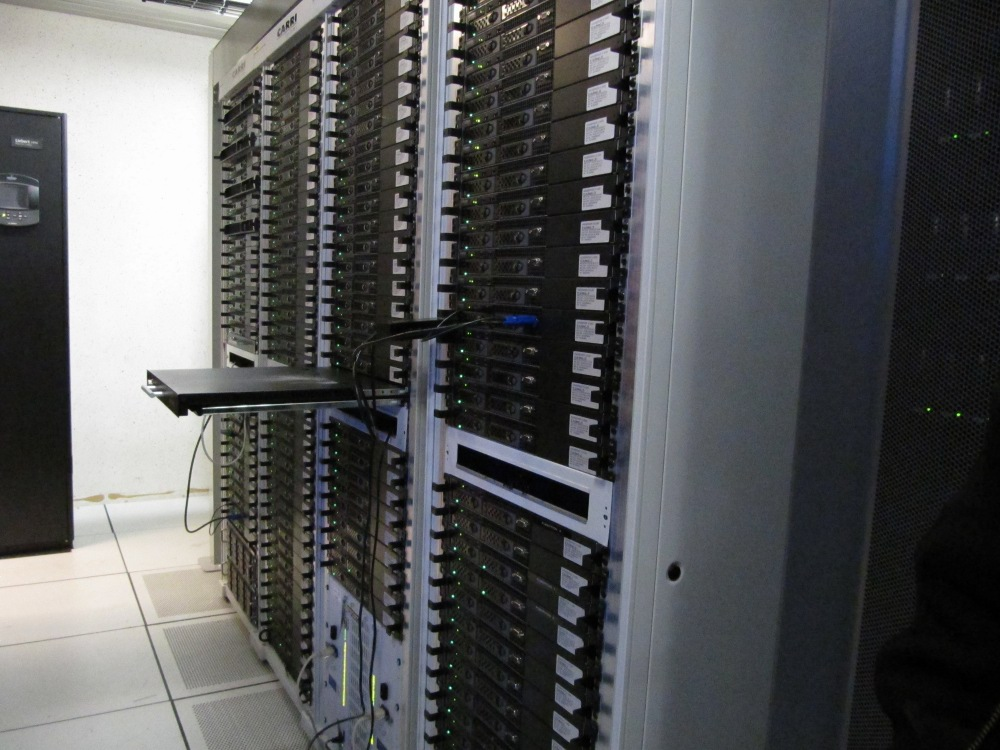
\includegraphics[width=0.6\linewidth]{images/cluster_nancy.jpg}
				\caption{Un cluster de Nancy}
			\end{center}
		\end{figure}
		


	\chapter{NFS}
		\section{Présentation}
		% FS distribué le plus simple ? (à mettre en place, dans ses possibilités) ?

NFS (Network File System, système de fichiers en réseau en français) est un système de fichiers développé par Sun Microsystem, permettant de partager des données par le réseau. NFS est aujourd’hui la méthode standard de partage de disques entre machines Unix. 
		C’est une solution simple et pratique, quoique peu sécurisée.\\
		
		\section{Aspect technique}
		
		NFS utilise généralement le protocole non connecté UDP (en opposition à TCP qui est un pro-
    tocole connecté). Toutefois, certains clients et serveurs NFS (depuis la version 3) peuvent aussi
    utiliser TCP, ce qui permet, entre autre, de fiabiliser les échanges.\\

    On retrouve pour NFS différentes versions :\\
    NFSv1 et v2 définies dans la RFC 1094 prévues pour fonctionner sur UDP.\\
    NFSv3 définie dans la RFC 1813 prenant en charge le TCP.\\
    NFSv4 définie dans la RFC 3010 puis réviser dans la RFC 3530. L'ensemble du protocole est repensé, et les codes sont réécrits.
    Cette version intègre une meilleur gestion de la sécurité, de la montée en charge, et un systèmes de maintenances simplifiés.
    NFSv4 supporte les protocoles de transports TCP (par défaut) et RDMA, ce qui augmente la fiabilité. Nous utiliserons donc cette version NFS dans l'ensemble de nos test.\\\\
Au delà des évolutions entre les versions 3 et 4 du protocole, c'est la cohérence du système de nommage qui distingue la version 4 du système de fichiers réseau. Il s'agit de garantir qu'un objet (fichier ou répertoire) est représenté de la même manière sur un serveur et sur ses clients.
\newpage

    \section{Mise en place}
Le rôle du serveur NFS est de mettre à disposition sur le réseau une partie de son arborescence locale de système de fichiers. On parle d'\og exportation\fg.\\
Il existe plusieurs implémentations libres de serveur NFS. On se limite ici à l'utilisation du logiciel lié au noyau Linux.\\
Dans cette configuration nous traitons de l'installation d'un serveur NFS en version 4 dont le but est d'exporter le contenu d'un répertoire /tmp vers les clients.
Utilisant une image de Debian Squeeze, On recherche dans la liste des paquets disponibles, ceux dont le nom débute par 'nfs'.
\begin{lstlisting}
# aptitude search ?name"(^nfs)"
v   nfs-client         -
i   nfs-common         - NFS support files common to client and server
i   nfs-kernel-server - support for NFS kernel server
v   nfs-server         -
p   nfs4-acl-tools     - Commandline and GUI ACL utilities for the NFSv4 client
p   nfswatch           - Program to monitor NFS traffic for the console
	  \end{lstlisting}
Dans la liste ci-dessus, on identifie les paquets nfs-common et nfs-kernel-server qui correspond bien aux fonctions souhaité pour le client et le serveur NFS.
En exploitant la documentation \href{https://wiki.linux-nfs.org/wiki/index.php/Nfsv4_configuration_fr}{Nfsv4 configuration} et l'exemple donné dans le fichier de configuration, on applique la configuration suivante dans le fichier /etc/exports :
    \begin{lstlisting}
	    /tmp *.nancy.grid5000.fr(rw,fsid=0,insecure,subtree_check)
	  \end{lstlisting}
Pour les besoins de ces travaux pratiques, les fonctions de sécurité Kerberos ne sont pas utilisées. On utilise l'appartenance au domaine nancy.grid5000.fr comme critère de contrôle d'accès ; ce qui correspond à un niveau de sécurité faible, puisque toutes les machines déployées sur la plateforme de Nancy peuvent accéder au répertoire.\\
	  \textbf{rw }: autorise les requêtes en lecture et écriture;\\
	  \textbf{fsid=0} : (fsid=root ou fsid=0) cette option est propre à NFSv4. Elle permet de définir le point de partage racine. Ce qui permet de monter des partages en fonction d'une racine virtuelle.\\
	  \textbf{insecure} : l'option insecure permet l'accès aux clients dont l'implémentation NFS n'utilisent pas un port réservé.\\
	  \textbf{subtree\_check} : permet de limiter l'accès exclusivement au répertoire partager.\\
	  
	  Après la modification de ce fichier, il suffit de redémarrer le service, puis de monter les clients sur le répertoire partager à l'aide de la commande suivante :\\
	  \begin{lstlisting}
	    mount serveur:/ -t nfs4 /tmp/partage
	  \end{lstlisting}
	  Afin d'utiliser la version 4 de NFS, il est nécessaire de le spécifier dans le type lors du montage.\\
Depuis le serveur, la commande exportfs est chargée de la gestion de la liste des systèmes de fichiers partagés. L'exécution de cette commande sans argument affiche la liste des répertoires exportés.
Ainsi on peut vérifier que les directives données dans le fichier /etc/exports sont effectivement appliquées.
Sur le client, nous avons le programme appelé showmount associé à l'option -e.

	  \chapter{Fuse}
    FUSE est un logiciel libre signifiant \og Filesystem in Userspace\fg. Il s'agit d'un module, disponible pour les kernels 2.4 et 2.6, grâce auquel 
    il est possible d'implémenter toutes les fonctionnalités d'un système de fichier dans un espace utilisateur. Ces fonctionnalités incluent :\\
	\begin{itemize}
		\item une API de librairie simple ;
		\item une installation simple (pas besoin de patcher ou recompiler le noyau) ;
		\item une implémentation sécurisée ;
		\item utilisable dans l'espace utilisateur.\\
   \end{itemize}

    Pour pouvoir monter un système de fichier, il faut être administrateur à moins que les informations de montage aient été renseignées sur le fichier /etc/fstab.\\
    FUSE permet à un utilisateur de monter lui-même un système de fichier. Pour profiter de FUSE, il faut des programmes qui exploitent sa bibliothèque
    et  ces programmes sont nombreux.\\
    http://fuse.sourceforge.net\\\\
    L'installation de FUSE est réalisé avec la commande suivante:\\
    \begin{lstlisting}
	  apt-get install fuse-utils libfuse2
	  \end{lstlisting}
    Avant de pouvoir utiliser ce paquet, il faut charger le module \og fuse\fg~ en mémoire :\\
    \begin{lstlisting}
	  modprobe fuse
	  \end{lstlisting}
    Pour charger le module automatiquement à chaque démarrage de l'ordinateur, il faut ajouter \og fuse\fg~ dans le fichier \og /etc/modules\fg.\\
    \begin{lstlisting}
	 nano /etc/modules
	 \end{lstlisting}

	\chapter{GlusterFS, véritable serveur d'archivage.}
		\section{Présentation}

		\begin{figure}[H]
			\begin{center}
				
\includegraphics[width=0.6\linewidth]{images/glusterfs.png}
			\end{center}
		\end{figure}

GlusterFS est un système de fichiers distribués libre (GPLv3), à la fois très simple à mettre en œuvre et dont les capacités de stockage peuvent monter jusqu'à plusieurs petabytes (1,000 milliards octets).\\
GlusterFS est composé de deux éléments logiciels : un serveur et un client.\\
GlusterFS supporte plusieurs protocoles de communication tels que TCP/IP, InfiniBand RDMA.\\

Les serveurs de stockage gèrent la réplication des données stockées dans le volume distribué, permettant une reprise rapide du service en cas d'indisponibilité de l'un des n\oe uds. \\
Les clients reposent sur Fuse pour monter localement l'espace de stockage fusionné, donc facilement administrable.\\
Le nombre de serveur et le nombre de clients ne sont pas limité.\\\\
Le fonctionnement de GlusterFS est très modulaire et peut être configuré pour :\\
	\begin{itemize}
		\item fusionner l'espace de tous les nœuds,
		\item assurer une redondance des données,
		\item découper les gros fichiers en tronçons plus petits qui seront répartis sur différents serveurs de stockage (stripping),
		\item fonctionner malgré la perte d'un ou plusieurs nœuds de stockage qui seront automatiquement réintégrée dans le cluster et resynchronisés dès qu'ils seront de nouveau actifs \dots \\
	\end{itemize}
\newpage

\section{Mise en place}
\textbf{Installation de GlusterFS}\\\\
Pour vous présenter la méthodologie d'installation des deux parties Serveur et Client, nous allons réaliser la plus simple architecture, à savoir deux serveurs qui abriterons le volume distribué et le montage de celle-ci par une machine cliente.\\
La distribution choisie est une Debian Squeeze pour l'ensemble de la maquette, et le choix des paquets glusterfs-server et glusterfs-client en version 3.1.2 officiellement stable.\\\\
Actuellement, l'ajout du dépôt Sid\footnote{Version de Debian \og instalble\fg~, en développement} est obligatoire pour pouvoir accès à cette version de Gluster.\\\\
Modification du fichier /etc/apt/sources.list pour l'ajout des dépôts de Debian Sid, suivi de la gestion des priorités /etc/apt/preferences.
\begin{lstlisting}
Ajout des depots Sid
deb http://ftp.fr.debian.org/debian squeeze main contrib
deb http://security.debian.org/ squeeze/updates main contrib
deb http://ftp.fr.debian.org/debian sid main contrib

gestion des priorites
Package: *
Pin: release a=stable
Pin-Priority: 700
Package: *
Pin: release a=unstable
Pin-Priority: 600
\end{lstlisting}
\textbf{Installation de GlusterFS Serveur}
Actualisez le contenu du catalogue de paquets, installez le module serveur sur les deux machines.
\begin{lstlisting}
aptitude update;aptitude install glusterfs-server/sid
Mettre a jour la librairie libglusterfs0 a partir de sid : 
aptitude install libglusterfs0/sid
	  \end{lstlisting}
Choix du paquet différent pour le client.
\begin{lstlisting}
aptitude update;aptitude install glusterfs-client/sid
Mettre a jour la librairie libglusterfs0 a partir de sid : 
aptitude install libglusterfs0/sid
	  \end{lstlisting}
Nous passons à la configuration du volume distribué. Nous créons un volume qui sera la concaténation des deux volumes offerts par nos deux serveurs.\\
Le montage du volume sera réalisé dans /sharespace, créons ce répertoire maintenant\\
\begin{lstlisting}
mkdir -p /sharespace
	  \end{lstlisting}
La génération des fichiers de configuration s'effectuera à partir de notre premier serveur grâce à la commande glusterfs-volgen.\\
Voila les IP que nous allons utiliser pour une meilleur compréhension :
	\begin{itemize}
		\item IP serveurs : 172.16.65.91 et 172.16.65.92
		\item IP cliente :  172.16.65.90\\
	\end{itemize}
\begin{lstlisting}
glusterfs-volgen --name mystore 172.16.65.92:/sharespace 172.16.65.91:/sharespace
\end{lstlisting}
Retour de serveur :
\begin{lstlisting}
Generating server volfiles.. for server '172.16.65.92'
Generating server volfiles.. for server '172.16.65.91'
Generating client volfiles.. for transport 'tcp'
	  \end{lstlisting}
Vous pouvez constater que la méthode de transport par défaut est le protocole TCP.\\\\
En cas d'infrastructure équipé de l'InfiniBand (bus à haut débit), nous aurions pu le définir à cette étape par le biais de l'option -t ib-verbs, sans oublier d'installer les librairies nécessaires. Nous aurions eu :\\
\begin{lstlisting}
apt-get install libibverbs1 librdmacm1
glusterfs-volgen --name mystore -t ib-verbs 172.16.65.92:/sharespace 172.16.65.91:/sharespace
	  \end{lstlisting}
La commande glusterfs-volgen génère les fichiers de configuration pour les serveurs et le client. Chaque fichier porte l'IP de la machine concerné dans son nom, nous allons les exporter dans leur répertoire d'exploitation et les renommer pour les qu'il soient pris en compte.
\begin{lstlisting}
cp 172.16.65.91-mystore-export.vol /etc/glusterfs/glusterfsd.vol
cp mystore-tcp.vol /etc/glusterfs/glusterfs.vol

pour le second serveur
scp 172.16.65.92-mystore-export.vol 172.16.65.92:/etc/glusterfs/glusterfsd.vol
scp mystore-tcp.vol 172.16.65.92:/etc/glusterfs/glusterfs.vol
	  \end{lstlisting}
Une copie du fichier de transport ou fichier de configuration client doit être stocké par au moins un serveur.\\
A ce moment, nous sommes êtes prêt à mettre en marche les services de GlusterFS sur chaque serveur :
\begin{lstlisting}
/etc/init.d/glusterfs-server start
	  \end{lstlisting}
Montage d'un poste client.\\\\
Petit aparté pour vous spécifier que le protocole en natif est fuse, mais que l'applicatif est capable de supporter d'autres protocoles, NFS, CIFS ou encore Dav.\\
Le paquet gluster étant installé, passons à la création du point de montage.
\begin{lstlisting}
mkdir -p /mnt/monglusterfsvolume
	  \end{lstlisting}
Notre client va maintenant monter le volume réparti, il suffit d'employer la commande mount.
\begin{lstlisting}
mount -t glusterfs 172.16.65.91:6996 /mnt/monglusterfsvolume/
	  \end{lstlisting}
Lors du montage, GlusterFS va initier une connexion vers le serveur spécifié afin de récupérer le fichier de configuration du client que nous avons stocké précédemment sous /etc/glusterfs/glusterfs.vol.\\\\
ATTENTION\\
Nous avons pu constater que cette étape ne fonctionnait pas toujours très bien. Cela a pour conséquence de générer des dysfonctionnements dues à des problèmes de droits. Nous aurons droit à la lecture et à la modification des fichiers présent dans le volume.\\
Pour résoudre cette mauvaise initialisation, copions le fichier de transport manuellement dans /etc/glusterfs/ et remontons le volume pour recharger le nouveau fichier de configuration avec la commande :
\begin{lstlisting}
mount -t glusterfs /etc/glusterfs/glusterfs.vol /mnt/monglusterfsvolume/
	  \end{lstlisting}
Pour le monter automatiquement à chaque démarrage, il faut ajouter la ligne suivante au fichier /etc/fstab
Pour un serveur :
\begin{lstlisting}
172.16.65.91  /mnt/monglusterfsvolume  glusterfs  defaults,_netdev  0  0
	  \end{lstlisting}
Pour un client :
\begin{lstlisting}
/etc/glusterfs/glusterfs.vol  /mnt/monglusterfsvolume  glusterfs  defaults,_netdev  0  0
	  \end{lstlisting}
Vérifions le volume :
\begin{lstlisting}
df -h /mnt/monglusterfsvolume
Filesystem            Size  Used Avail Use% Mounted on
/etc/glusterfs/glusterfs.vol
                      9.4G  831M  8.1G  10% /mnt/monglusterfsvolume
	  \end{lstlisting}
ou encore
\begin{lstlisting}
df -h | grep 172.16.65.91
172.16.65.91 5.6G 2.1G 3.3G 39% /mnt/monglusterfsvolume
	  \end{lstlisting}
A des fins de test, concevons un fichier de 10 Mo
\begin{lstlisting}
dd if=/dev/urandom of=test bs=10M count=1
1+0 enregistrements lus
1+0 enregistrements ecrits
10485760 octets (10 MB) copies, 1,45815 s, 7,2 MB/s
	  \end{lstlisting}
Copions le fichier test sur le FS distribué :
\begin{lstlisting}
cp test /mnt/monglusterfsvolume
	  \end{lstlisting}
Examinons le contenu des répertoires /mnt/monglusterfsvolume et /sharespace des deux serveurs.\\
ls -lh /mnt/monglusterfsvolume\\
ls -lh /sharespace\\
On constate l'absence du fichier test sur l'un des nœuds, ce qui est totalement cohérent puisque la configuration par défaut de GlusterFS est la mise en œuvre de la concaténation des volumes physiques et sans duplication ou réplication des données.\\
Nous utilisons donc l'espace des deux volumes sur les serveurs, qui est vu comme un seul par les clients.
Vous trouverez ci-dessous des informations complémentaires sur les possibilités des fichiers de configuration même si nous n'y toucherons pas pour notre travail.\\
\newpage
Listing du fichier glusterfsd.vol
\begin{lstlisting}
volume posix
     type storage/posix
     option directory /mount/glusterfs
end-volume
volume plocks
 type features/posix-locks
 subvolumes posix
end-volume
volume brick
 type performance/io-threads
 option thread-count 4
 option cache-size 64MB
 subvolumes plocks
end-volume
volume brick-ns
     type storage/posix
     option directory /mount/glusterfs-ns
end-volume
volume server
     type protocol/server
     option transport-type tcp/server
     option listen-port 6996
     option bind-address 127.0.0.1
     subvolumes brick brick-ns
     option auth.ip.brick.allow 127.0.0.1
end-volume
	  \end{lstlisting}
Le module “posix” pointe vers l'espace de stockage des données “/mount/glusterfs”.\\
Le module “plocks” hérite du module “posix” et y ajoute de verrous de fichiers.\\
Le module “brick” hérite du module “plocks” et y ajoute un cache en lecture.\\
Le module “brick-ns” pointe vers l'espace de stockage de l'annuaire de fichiers (”namespace”) “/mount/glusterfs-ns”.\\
Le module “server” hérite des modules “bricks” et “brick-ns” et les publie sur le port TCP 6996 et pour le PC “localhost” uniquement.\\
Nous aurions par exemple pu ajouter un cache en écriture et un cache en lecture/écriture sur “brick-ns”.\\\\
Il est toujours primordial de bien définir le niveau de log :
\begin{lstlisting}
glusterfsd -f server1.vol -L DEBUG -l server1.log
glusterfsd -f server2.vol -L DEBUG -l server2.log
	  \end{lstlisting}
L'option \og -f\fg~ pointe vers le fichier de configuration, \og -L\fg~  indique le niveau de journalisation souhaité et \og -l\fg~ donne le nom du fichier de journaux par
instance de \og GlusterFS\fg.\\\\
\newpage
Listing du fichier /etc/glusterfs/client.vol.
\begin{lstlisting}172.16.65.91
### Ajoutez la caracteristique du client et rattachez au subvolume des servers
volume brick1
type protocol/client
option transport-type tcp/client
option remote-host 172.16.65.91    
option remote-subvolume brick       
end-volume

volume brick2
type protocol/client
option transport-type tcp/client
option remote-host 172.16.65.92
option remote-subvolume brick      
end-volume

### Fichier d'index du serveur1
volume brick1-ns
type protocol/client
option transport-type tcp/client
option remote-host 172.16.65.91 
option remote-subvolume brick-ns  
end-volume

### Fichier d'index du serveur2
volume brick2-ns
type protocol/client
option transport-type tcp/client
option remote-host 172.16.65.92 
option remote-subvolume brick-ns
end-volume
 
###Volume repique pour les donnees
volume afr1
type cluster/afr
subvolumes brick1 brick2
end-volume
 
###Volume repique pour les index
volume afr-ns
type cluster/afr
subvolumes brick1-ns brick2-ns
end-volume
 
###Unification des volumes afr (utilises quans il y a plus de deux serveurs)
volume unify
type cluster/unify
option scheduler rr # round robin
option namespace afr-ns
subvolumes afr1
end-volume
	  \end{lstlisting}
Un dialogue est établi entre le client et les serveurs par le port par défaut de glusterts : 6996. Les espaces de stockage nommés \og brick\fg~ de chacun de ses serveurs seront fusionnés par le module \og cluster/unify\fg.\\ L'amélioration des performances passe par l'écriture à tour de rôle vers les différents serveurs ; vous aurez reconnu l'utilisation de l'algorithme de répartition de charge round robin (rr).\\
Les données de l'annuaire de données quand à elles sont écrites en parallèle sur les espaces de stockage \og brick-ns\fg, directive du module \og cluster/afr\fg.\\\\
Nous pourrions rajouter des directives à des fins de performances, voici un exemple:
\begin{lstlisting}
volume iot
 type performance/io-threads
 option thread-count 2
 subvolumes bricks
end-volume

### Ajout de la directive writebehind pour la structure de donnees
volume writebehind
type performance/write-behind
option aggregate-size 131072 # unite en bytes
subvolumes iot
end-volume

### Ajout de la directive readahead pour la structure de donnees
volume readahead
 type performance/read-ahead
 option page-size 65536   # unit in bytes
 option page-count 16     # cache per file = (page-count x page-size)
 subvolumes writebehind
end-volume
	  \end{lstlisting}

Le tableau suivant répertorie les options de volume ainsi que sa description et la valeur par défaut (d'autres options existent):\\\\
\begin{tabular}{|p{5cm}|p{8cm}|m{4cm}|}
  \hline
  Option & Description & Valeur par défaut \\
  \hline
  performance.cache-refresh-timeout & Les données mises en cache pour un fichier sera conservé x secondes, après quoi revalidation des données est effectuée. & 1 sec \\
  \hline
  performance.cache-size & Taille du cache de lecture. & 32 MB \\
  \hline
  performance.write-behind-window-size & taille du per-file écrire dérriere le buffer & 1 MB \\
  \hline
  network.frame-timeout & Le délai après lequel l'opération doit être déclaré comme mort, si le serveur ne répond pas à une opération particulière. & 1800 (30 mn) \\
  \hline
  network.ping-timeout & La durée pendant laquelle le client attend de vérifier si le serveur est sensible. & 42 secs  \\
  \hline
  auth.allow & Les adresses IP ou nom d'hôte qui devraient être autorisés à accéder au volume & * (permis à tous) \\
  \hline
  auth.reject & Les adresses IP ou nom d'hôte qui devraient se voir refuser l'accès au volume. & NONE (aucun rejet) \\
  \hline
  diagnostics.brick-log-level & Changements du niveau de journalisation des serveurs. & NORMAL \\
  \hline
  diagnostics.client-log-level & Changements du niveau de journalisation des clients & NORMAL \\
  \hline
  
\end{tabular}

	\chapter{MooseFS}
		% données temporaires, penser à citer les sources si passages copiés collés
		% il est apparemment aussi possible de mettre en place MooseFS sur un seul serveur
		\section{Présentation}

			\begin{figure}[H]
				\begin{center}
					
\includegraphics[width=0.15\linewidth]{images/moosefs.png}
				\end{center}
			\end{figure}
	
			%MooseFS (Moose File System), un système de fichiers distribué. % enlever cette phrase ?
				
			MooseFS (Moose File System) est un système de fichiers répartis à tolérance de panne,
			c’est à dire résistant aux pannes d’un ou plusieurs nœuds de stockage.
			Développé par Gemius SA. Le code préalablement propriétaire a été libéré et mis à disposition publiquement le 5 mai 2008
			sous licence GPLv3. Disponible pour Linux, FreeBSD, OpenSolaris et MacOS X.

			Les développeurs sont réactifs et suivent de très près la liste de diffusion et les remontés de bugs de leurs utilisateurs.

			MooseFS permet de déployer assez facilement un espace de stockage réseau, répartit sur plusieurs serveurs. 
			Les fichiers sont découpés en morceaux (appelés chunks) puis répartis sur les différents chunkservers (nœuds de stockage) :
			selon le paramétrage voulu pour ces fichiers, ou pour le répertoire dans lequel ils se trouvent,
			chaque chunk sera répliqué sur x noeuds (différents).

			Cette répartition permet de gérer la disponibilité des données, lors des montées en charge ou lors d’incident technique
			sur un serveur. L'atout principal de MooseFS, au-delà du fait qu'il s’agisse d’un logiciel libre,
			est sa simplicité d'administration et sa de mise en œuvre.\\
			% plus simple à mettre en place que les autres ?

			D'autres qualités sont à son actif:
			\begin{itemize}
                          \item Le respect de la norme Posix.
			  \item L'utilisation de Fuse en espace client.
			  \item La mise à disposition d'une poubelle automatique à durée de rétention modifiable à souhait.
			  \item Une commande unique « mfssetgoal », à chaud pour le choix du nombre de répliquas, par fichier ou par répertoire. Disponibilité des données ou tolérance aux pannes en cas de réplication positionné à plus de 1 pour les données rendra transparent la perte d'un chunkserver au détriment d'un coût en matière de place.
			  \item Simplicité de l'extension de l'espace de stockage à chaud quelque soit la configuration, comprenant la ré-indexation et la répartition des données vers ces nouveaux espaces avoir à intervenir (cela peut prendre plusieurs heures).
			  \item Le système est réparti: les fichiers supérieurs à 64Mo sont découpés en paquets de 64Mo et distribués sur les différents serveurs de données dit « chunkserver ».
                        \end{itemize}

			\section{Aspect technique}
				
				Les montage du système de fichiers par les clients se fait à l'aide de FUSE.
				MooseFS est constitué de trois types de serveurs :

				\begin{enumerate}
					\item Un serveur de métadonnées (MDS)

					Ce serveur gère la répartition des différents fichiers
					\item Un serveur métajournal (Metalogger server)

					Ce serveur récupère régulièrement les métadonnées du MDS et les stocke en tant que sauvegarde.
					\item Des serveurs Chunk (CSS) % pourquoi CSS ?

					Ce sont ces serveurs qui stockent les données des utilisateurs.
				\end{enumerate}
				
				Le point le plus important étant de bien dimensionner le serveur Master (qui stocke les méta-données)
				afin de ne pas être limité par le suite.\\

				MooseFS permet de partager des données sur plusieurs machines de manière rapide, fiable et sécurisée.

		\section{Mise en place}

Le système utilisé est une Debian Squeeze. MooseFs ne faisant pas partie des dépôts de la distribution, nous avons compilé le paquet à partir des sources dans la dernière version disponible (1.6.20) sur le site officiel.\\
\href{http://pro.hit.gemius.pl/hitredir/id=0sWa0S8ft4sTAHF1bGAAEZPcP3ziyq7f9SdhoQf7oeT.c7/url=moosefs.org/tl\_files/mfscode/mfs-1.6.20-2.tar.gz}{http://www.moosefs.org/download.html} \\\\

Méthodologie d'installation pour la mise en œuvre des différents serveurs ou services sur des machines dédiées :\\\\
Commençons par \textbf{l'installation d'un Master serveur}\\\\
Récupérons l'archive sur le site de MooseFs et décompressons la dans le répertoire /usr/src/,\\ tar zxvf mfs-1.6.20-2.tar.gz\\
Pour des questions d'isolement nous créons un utilisateur et un groupe pour faire tourner le futur service.\\
\begin{lstlisting}
	  groupadd mfs;useradd mfs -s /sbin/nologin
	  \end{lstlisting}
Positionnons nous dans le répertoire de l'archive, cd /usr/src/mfs-1.6.20-2\\
Nous compilons avec la prise en compte de notre nouveau utilisateur et nous désactivons les services non nécessaire à notre master.
Désactivation du service mfschunck (stockage de données) et mfsmount (montage côté client)
\begin{lstlisting}
./configure --prefix=/usr --sysconfdir=/etc --localstatedir=/var/lib --with-default-user=mfs --with-default-group=mfs --disable-mfschunkserver --disable-mfsmount
	  \end{lstlisting}
\begin{lstlisting}
	   make;make install
	  \end{lstlisting}
Nous recopions les fichiers exemples du répertoire /etc pour la configuration du service, au nombre de trois:
\begin{lstlisting}
cd /etc
cp mfsmaster.cfg.dist mfsmaster.cfg
cp mfsmetalogger.cfg.dist mfsmetalogger.cfg
cp mfsexports.cfg.dist mfsexports.cfg
	  \end{lstlisting}
Si nous ne modifions pas ces fichiers, les directives par défaut seront alors appliquées.
Pour information toutes les directives sont très bien documenté dans le page de man (exp: man mfsmaster.cfg).\\
Nous ne toucherons pas au fichier mfsmaster.cfg, celui-ci défini les principaux arrangements du serveur.
Nous adaptons la configuration du fichier mfsexports.cfg qui permet de fixer la plage d'IP ou les ordinateurs qui pourrons monter le système de fichiers et de convenir des privilèges.
La première ligne non commenté nous intéresse, nous remplaçons l'astérisque (*) en spécifions la plage IP et son masque que nous allons employer pour notre maquette.
Cela aura pour effet de donner accès à toutes les machines de cette plage d'IP à la totalité de la structure en mode lecture écriture.\\
Exemple de la ligne modifié :
\begin{lstlisting}
	  192.168.2.0/24 / rw,alldirs,maproot=0
	  \end{lstlisting}
Les binaires de méta-données et les fichiers de changelog sont maintenus dans un dossier spécifié lors de la compilation /var/lib, mais lors de l'installation le fichier de metadata est initialisé vide.
Nous allons changer cela: 
\begin{lstlisting}
cd /var/lib/mfs
cp metadata.mfs.empty metadata.mfs
	  \end{lstlisting}
Avant le démarrage du service nous devons penser à la résolution de nom du serveur. Renseigné votre DNS\footnote{Domaine Name Serveur : serveur de noms}, nous renseignons dans notre fichier hosts.
A titre d'exemple:
  \begin{lstlisting}
192.168.1.1 mfsmaster
	  \end{lstlisting}
A ce stade nous pouvons démarrer le master serveur, le service démarrera avec le compte mfs
  \begin{lstlisting}
usr/sbin/mfsmaster start
	  \end{lstlisting}
En cas de mise en production pensez à modifier votre configuration pour un démarrage automatique du service lors des lancements de votre serveur.

Pour conclure cette section, un mode graphique en cgi\footnote{Common Gateway Interface : interface utilisée par les serveurs HTTP} est disponible pour suivre l'état de fonctionnement du système, disponible sous votre navigateur à l'adresse http://IP\_Master\_Server:9425
  \begin{lstlisting}
/usr/sbin/mfscgiserv
	  \end{lstlisting}
Remarque: le contenu sera vide tant que les serveurs de données ne seront pas démarrés.\\\\
				% avec options différentes suivant les serveurs, clients (cf tuto site officiel)
\newpage
\textbf{Installation du Serveur de Backup Metalogger.}\\\\
Le principe de ce serveur est la de récupérer tous les événements du système de fichier et peut permettre, si le maître est vraiment mal en point (perte de ses metadada, ou de son historique), de lui faire rejouer les logs pour que le volume reste cohérent.\\
Cette solution repose sur le protocole Carp \og Common Address Redundancy Protocol\fg, permet d'admettre à un groupe d'hôtes sur le même segment réseau (ici mfsmaster et mfsmetalogger) de partager même adresse IP (un maître et un esclave). 
La méthodologie d'installation est similaire au master serveur.\\
Voici les commandes à suivre :\\
  \begin{lstlisting}
groupadd mfs
useradd -g mfs mfs
cd /usr/src
tar -zxvf mfs-1.6.20-2.tar.gz
cd mfs-1.6.20-2
	  \end{lstlisting}
Désactivation du service mfschunck (stockage de données) et mfsmount (montage côté client)
  \begin{lstlisting}
./configure --prefix=/usr --sysconfdir=/etc --localstatedir=/var/lib --with-default-user=mfs --with-default-group=mfs --disable-mfschunkserver --disable-mfsmount
make;make install
cd /etc
cp mfsmetalogger.cfg.dist mfsmetalogger.cfg
	  \end{lstlisting}
Déclarer le serveur master auprès de votre fichier /etc/hosts: 192.168.1.1  mfsmaster\\
Le démarrage automatique n'est pas configuré. Commande de lancement :
  \begin{lstlisting}
/usr/sbin/mfsmetalogger start
	  \end{lstlisting}
\textbf{Installation d'un Serveur de Données Chunk servers.}\\\\
Procédure d'installation toujours similaire:\\
Désactivation du service mfsmaster\\
  \begin{lstlisting}
groupadd mfs
useradd -g mfs mfs
cd /usr/src
tar -zxvf mfs-1.6.20-2.tar.gz
cd mfs-1.6.20-2
./configure --prefix=/usr --sysconfdir=/etc --localstatedir=/var/lib --with-default-user=mfs --with-default-group=mfs --disable-mfsmaster
make;make install
	  \end{lstlisting}
Préparation des fichiers de configurations:\\
  \begin{lstlisting}
cd /etc/
cp mfschunkserver.cfg.dist mfschunkserver.cfg
cp mfshdd.cfg.dist mfshdd.cfg
	  \end{lstlisting}
Les directives du fichier mfshdd.cfg signalent les emplacements des unités de disque dur que l'on souhaite employer.\\\\
Exemple de mise en œuvre pour deux emplacements :\\
Ajoutons les deux lignes suivantes dans le fichier mfshdd.cfg.\\
/mnt/mfschunks1\\
/mnt/mfschunks2\\
Positionnons les droits d'écriture nécessaire pour la création des dossiers de .lock :\\
  \begin{lstlisting}
mkdir /mnt/mfschunks1
mkdir /mnt/mfschunks2
chown -R mfs:mfs /mnt/mfschunks1
chown -R mfs:mfs /mnt/mfschunks2
	  \end{lstlisting}
Si nous ne souhaitons pas utiliser la totalité de l'espace libre de vos disques, nous pouvons utiliser une autre méthode permettant de contrôler le volume disque.\\
Création et formatage d'un volume de deux gigas et d'un formatage en ext3.\\
  \begin{lstlisting}
dd if=/dev/zero of=disk1 bs=1024 count=1 seek=$((2*1024*1024-1))
dd if=/dev/zero of=disk2 bs=1024 count=1 seek=$((2*1024*1024-1))
mkfs -t ext3 disk1
mkfs -t ext3 disk2
	  \end{lstlisting}
Nous montons nos nouveaux disques, sans oublier les droits d'écriture.\\
  \begin{lstlisting}
mkdir /mnt/hd1
mkdir /mnt/hd2
mount -t ext3 -o loop disk1 hd1
mount -t ext3 -o loop disk2 hd2
chown -R mfs:mfs /mnt/hd1
chown -R mfs:mfs /mnt/hd2
	  \end{lstlisting}
Nous informons le fichier /etc/hosts de la présence du master serveur : 192.168.1.1 mfsmaster\\
Il est prêt à être démarrer:
  \begin{lstlisting}
/usr/sbin/mfschunkserver start
	  \end{lstlisting}
\textbf{Installation d'un Poste Client.}\\\\
Afin de monter le système de fichiers basé sur Fuse, la version du paquet doit être égal ou supérieur à 2.7.2\\
\href{http://sourceforge.net/projects/fuse/}{http://sourceforge.net/projects/fuse/} \\
Compilation de Fuse et chargement du module du noyau linux.\\
  \begin{lstlisting}
cd /usr/src
tar -zxvf fuse-2.8.5.tar.gz
cd fuse-2.8.5
./configure;make;make install
modprobe fuse
	  \end{lstlisting}
\newpage
Afin d'installer le service mfsmount nous réalisons les étapes suivantes :
  \begin{lstlisting}
tar -zxvf mfs-1.6.20-2.tar.gz
cd mfs-1.6.20-2
./configure --prefix=/usr --sysconfdir=/etc --localstatedir=/var/lib --with-default-user=mfs --with-default-group=mfs --disable-mfsmaster --disable-mfschunkserver
make;make install
	  \end{lstlisting}
Nous annonçons le master serveur au fichier /etc/hosts : 192.168.1.1   mfsmaster\\
Supposons que nous souhaitons monter le système dans le dossier /mnt/mfs notre machine de cliente.\\
  \begin{lstlisting}
mkdir -p /mnt/mfs
chown -R mfs:mfs /mnt/mfs
/usr/bin/mfsmount /mnt/mfs -H mfsmaster
	  \end{lstlisting}
Nous pouvons vérifier l'espace occupé par les systèmes de fichiers avec la commande df, option h améliora la lisibilité.\\
exemple : df -h | grep mfs\\
  \begin{lstlisting}
/storage/mfschunks/mfschunks1
                      2.0G   69M 1.9G 4% /mnt/mfschunks1
/storage/mfschunks/mfschunks2
                      2.0G   69M 1.9G 4% /mnt/mfschunks2
mfs#mfsmaster:9421    3.2G     0 3.2G 0% /mnt/mfs
	  \end{lstlisting}
\textbf{Commandes Usuelles}\\\\
Montage de la Poubelle :\\
\begin{lstlisting}
mkdir -p /mnt/mfsmeta
chown -R mfs:mfs /mnt/mfsmeta
mfsmount -m /mnt/mfsmeta
	  \end{lstlisting}
Le temps est indiqué en secondes (valeurs utiles : 1 heure égal à 3600 secondes, 24h = 86400 secondes, 1 semaine = 604800 secondes).\\
Si nous définissons la valeur à 0 cela signifie une suppression immédiate du dossier et sa récupération ne sera plus possible. \\
Positionnons la rétention désiré pour la corbeille mfssettrashtime (option r permet la récursivité sur les répertoires) et vérifions la rétention appliqué mfsgettrashtime:
\begin{lstlisting}
mfsgettrashtime -r /mnt/mfs-test/test2
/mnt/mfs-test/test2:
files with trashtime 0 : 36
directories with trashtime 604800 : 1

mfssettrashtime -r 1209600 /mnt/mfs-test/test2
/mnt/mfs-test/test2:
inodes with trashtime changed: 37
inodes with trashtime not changed: 0
inodes with permission denied: 0

mfsgettrashtime -r /mnt/mfs-test/test2
/mnt/mfs-test/test2:
files with trashtime 1209600 : 36
directories with trashtime 1209600 : 1
	  \end{lstlisting}
Définissons le nombre de copies que l'on désir par répertoire avec le commande mfssetgoal –r :
\begin{lstlisting}
 mfssetgoal -r 1 /mnt/mfs/folder1
/mnt/mfs/folder1:
 inodes with goal changed:        0
 inodes with goal not changed:    1
 inodes with permission denied:   0

Remarquer la valeur 2 qui suit l'option -r qui 
permet de fixer le nombre de copie a 2

mfssetgoal -r 2 /mnt/mfs/folder2
/mnt/mfs/folder2:
 inodes with goal changed:        0
 inodes with goal not changed:    1
 inodes with permission denied:   0
	  \end{lstlisting}
Vérifions la redondance avec la fonction mfsgetgoal:
\begin{lstlisting}
mfsgetgoal /mnt/mfs/folder1
/mnt/mfs/folder1: 1

mfssetgoal /mnt/mfs/folder2
/mnt/mfs/folder2: 2
	  \end{lstlisting}
Le nombre réel de copies d'un dossier peut être vérifié avec les commandes mfscheckfile et de mfsfileinfo :
\begin{lstlisting}
mfscheckfile /mnt/mfs/folder1

/mnt/mfs/folder1:
3 copies: 1 chunks


mfsfileinfo /mnt/mfs/folder1

/mnt/mfs/folder1:
chunk 0: 00000000000520DF_00000001 / (id:336095 ver:1)
copy 1: 192.168.0.12:9622
copy 2: 192.168.0.52:9622
copy 3: 192.168.0.54:9622
\end{lstlisting}
Testons le positionnement:
\begin{lstlisting}
cp /usr/src/mfs-1.6.20-2.tar.gz /mnt/mfs/folder1
cp /usr/src/mfs-1.6.20-2.tar.gz /mnt/mfs/folder2
	  \end{lstlisting}
\newpage
La commande mfscheckfile est employée pour la vérification du nombre de copies :
\begin{lstlisting}
mfscheckfile /mnt/mfs/folder1/mfs-1.6.20-2.tar.gz
/mnt/mfs/folder1/mfs-1.6.20-2.tar.gz:
1 copies: 1 chunks

mfscheckfile /mnt/mfs/folder2/mfs-1.6.20-2.tar.gz
/mnt/mfs/folder2/mfs-1.6.20-2.tar.gz:
2 copies: 1 chunks
	  \end{lstlisting}
Le résumé du contenu de l'arbre entier du file systeme peut être appelé avec la commande mfsdirinfo :
\begin{lstlisting}
mfsdirinfo /mnt/mfs/folder1/:
inodes: 15
directories: 4
files: 8
chunks: 6
length: 270604
size: 620544
realsize: 1170432
	  \end{lstlisting}
\textbf{Arrêt de MooseFS}\\
\begin{lstlisting}
umount /mnt/mfs)
/usr/sbin/mfschunkserver stop
/usr/sbin/mfsmetalogger stop
/usr/sbin/mfsmaster stop
	  \end{lstlisting}
Discution général.\\
Dans tous les systèmes de fichiers contemporains, les fichiers sont écrits par le biais d'un buffer (cache d'écriture). En conséquence, l'exécution de la requête d'écriture elle-même transfère seulement les données au buffer (cache), l'écriture réelle n'ayant donc pas lieu. Conséquence, la confirmation de la requête d'écriture ne signifie pas que les données ont été correctement écrites sur un disque.\\ Elle est seulement invoquer et l'aboutissement passe par la commande fsync qui provoque le déchargement de toutes les données gardées en cache pour obtenir écrite physique sur le disque. Problématique en cas d'erreur avant la finalisation de cette phase, c'est un retour d'erreur de la commande fsync, voir la perte des données. 

	\chapter{Ceph}
		\section{Présentation}

                        \begin{figure}[H]
				\begin{center}
					
\includegraphics[width=0.40\linewidth]{images/cephfs.jpg}
				\end{center}
			\end{figure}-k -e squeeze-collective -u flevigne

                        CephFS est un système de fichiers distribué sous Licence LGPL, créé initialement par Sage Weill en 2007 pendant ses étude à l'université de Californie à Santa Cruz. Le but principal de CephFS est d'être compatible POSIX et d'être complètement distribué sans un seul point de défaillance. Les données sont répliqué de façon transparente ce qui fait de CephFS un système tolérant aux pannes. Mais CephFS est encore en phase de développement et il est fortement conseillé de ne pas l'utiliser en production.\\

                        Tout comme avec MooseFS les données sont découpées, réparties sur les différents serveurs et répliquées sur x nœuds. Cette répartition permet à CephFS d'avoir une grande tolérance vis-à-vis de la perte de nœuds stockant les données. De plus CephFS permet de rajouter ou d'enlever des serveurs de données pendant le fonctionnement de CephFS sans être obligé de couper le service.\\

                        CephFS remplit deux lacunes importantes des systèmes de fichiers actuellement disponible :
                        \begin{itemize}
                          \item robustesse du stockage distribué open-source. CephFS fournit une variété de fonctionnalités clés, généralement manquante dans les systèmes de fichiers open-s-k -e squeeze-collective -u flevigneource, tel que l'évolutivité transparente (capacité d'ajouter simplement un disque pour étendre le volume de stockage), la répartition de charge intelligente
                          \item évolutivité en terme de charge de travail ou de capacité de stockage. CephFS a été créer pour supporter des charges de l'ordre de dizaines de milliers de clients accédant au même fichier ou au même dossier. La capacité de stockage va du gigaoctet au petaoctet\footnote{1 petaoctet = 1024 teraoctet} et au-delà.
                        \end{itemize}
\newpage
                        
                \section{Aspect technique}
                        
                        La partie serveur de CephFS utilise trois types distinct de démons : 
                        \begin{itemize}
                        \item moniteur de cluster, qui garde trace des nœuds actifs et défaillants
                          \item serveurs de métadonnées, qui stockent les métadonnées des inoeuds et des répertoires
                          \item serveurs de données, qui stockent les données.
                        \end{itemize}

                        \subsection{Moniteur de cluster}
                           Le moniteur gère l'administration centrale, la configuration et l'état du cluster. C'est à partir du moniteur que l'on modifie le cluster : ajout ou suppression de serveurs de données et métadonnées. Les clients ont accès au données gérées par CephFS par l'intermédiaire d'un moniteur. Il garde en mémoire une carte du cluster, ce qu'il lui permet de communiquer aux clients sur quels serveurs de métadonnées et de données se connecter pour modifier, ajouter ou supprimer des fichiers.

                        \subsection{Serveurs de métadonnées}
                           Le démon gérant les serveurs de métadonnées agit en tant que cache cohérent et distribué du système de fichiers. Il contient les données concernant l'arborescence des fichiers et leurs métadonnées (nom, taille, emplacement mémoire sur les serveur de données). Avoir plusieurs serveurs de métadonnées a un certain avantage car cela permet d'équilibrer la charge de travail entre les différents serveurs et donc de gérer plus de clients au même moment.

                        \subsection{Serveurs de données}
                           Les serveurs de données stockent les fichiers du cluster. Ils sont découpés en morceaux et répliqués plusieurs fois sur des serveurs différents. Cela permet une certaine tolérance vis-à-vis de la perte de serveurs. Si jamais un serveur tombe en panne, les données sont toujours accessible car elles sont présente sur un autre serveur de données.


		        \begin{figure}[H]
			        \begin{center}
				        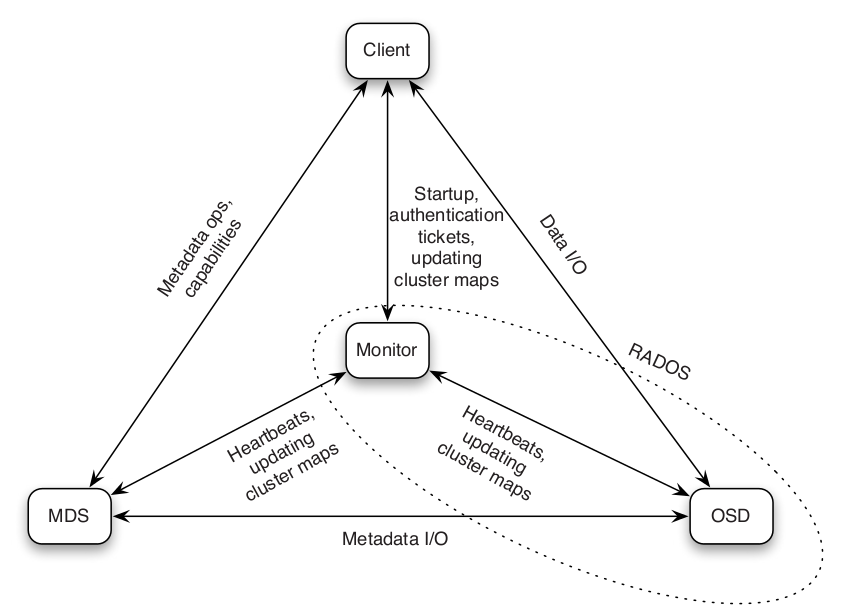
\includegraphics[width=0.61\linewidth]{images/Ceph_architecture2.png}
				        \caption{Fonctionnement de CephFS}
			        \end{center}
		        \end{figure}
		        \section{Mise en place}
		                       Avant toute configuration, il nous faut déterminiez les paquets qui nous seront utiles.Utilisant une image de Debian Squeeze, On recherche dans la liste des paquets disponibles, ceux dont le nom débute par 'ceph'.
		                       \begin{lstlisting}
# aptitude search ?name"(^ceph)
i   ceph                   - distributed storage and file system                                         
i A ceph-client-tools      - utilities to mount a ceph filesystem with the kernel client                 
p   ceph-client-tools-dbg  - debugging symbols for ceph-client-tools                                     
p   ceph-dbg               - debugging symbols for ceph                                                  
i A ceph-fuse              - FUSE-based client for the Ceph distributed file system                      
p   ceph-fuse-dbg          - debugging symbols for ceph-fuse
                           \end{lstlisting}	                       
		                       Afin de mettre en place Ceph, il faut connaitre le nombre exacte de serveurs qui seront utilisés. Dans cet exemple de mise en place, nous prenons deux serveurs, node0 et node1. node0 sera le serveur principal, que l'on appel aussi moniteur. La totalité de la configuration, hormis le montage des clients, se fait à partir du moniteur. Pour commencer, il faut créer un fichier de configuration ceph.conf qui contiendra une grande partie des données nécessaires au bon fonctionnement des serveurs :
		           \begin{lstlisting}
[global]
       pid file = /var/run/ceph/$name.pid
       debug ms = 1
       keyring = /etc/ceph/keyring.bin
[mon]
       mon data = /tmp/partage/mon$id
[mon0]
       host = node0
       mon addr = 10.0.0.10:6789
[mds]
       debug mds = 1
       keyring = /etc/ceph/keyring.$name
[mds0]
       host = node0
[mds1]
       host = node1
[osd]
       sudo = true
       osd data = /tmp/partage/osd$id
       keyring = /etc/ceph/keyring.$name
       debug osd = 1
       debug filstore = 1
       osd journal = /tmp/partage/osd$id/journal
       osd journal size = 1000
[osd0]
       host = node0
[osd1]
       host = node1

		           \end{lstlisting}           


	\chapter{Comparaison}
	% comparaison des performances
	% aspects générales, site officiel (doc, tuto), avis personnels
		\section{Test de performances}
			Afin de ne pas avoir de différence de matériel lors nos test, ceux-ci ont tous été réalisés sur un même cluster du Grid'5000 : Graphene.\\

			Ce cluster est composé de 144 noeuds, avec pour caractéristique :
			\begin{itemize}
				\item 1 CPU Intel de quatre cœurs cadencé à 2.53 GHz
				\item 16 Go de RAM
				\item 278 Go d'espace disque\\
			\end{itemize}

			Nous avons développé un benchmark mesurant les performances (débit) de quatre type d'opérations sur le système de fichier distribué :
			\begin{description}
				\item[Écriture de petits fichiers :] écriture des sources du noyau linux (décompressé).
				\item[Écriture de gros fichiers :] écriture de trois fichiers de 1 Go
				\footnote{Fichier créé avec la commande : dd if=/dev/urandom of=/lieu/voulu bs=1G count=1}. Les trois fichiers sont différents.
				\item[Lecture de petits fichiers: ] lecture des fichiers du noyau linux.
				Pour cela, nous avons compressé le dossier contenant le noyau (impliquant la lecture des fichiers),
				en redirigeant la sortie vers /dev/nul (afin que les performances du disque ne rentrent pas en jeux).
				\item[Lecture de gros fichiers :] lecture des fichiers de 1 Go. Opération réalisé en faisant un "cat" des fichier,
				et en redirigeant la sortie vers /dev/nul afin de ne pas \og polluer\fg~le terminal.\\
			\end{description}

			Les scripts de benchmark se découpent en deux parties :
			\begin{description}
				\item[Quatre petits scripts Bash]décrivant les opérations à réaliser, décrite ci dessus.
				\item[Un script écrit en Ruby] contrôlant l'ensemble du benchmark.
				Ce script se charge de distribuer les scripts Bash aux clients par SCP
				\footnote{Secure copy : désigne un transfert sécurisé de fichiers entre deux ordinateurs utilisant le protocole de communication SSH (Wikipédia)},
				et leur demande de les exécuter. Afin que l'ensemble des clients effectuent ces opérations simultanément, il a fallu mutlithreader le script
				(en utilisant la fonction fork\footnote{Cette fonction permet à un processus de donner naissance à un nouveau processus,
				par exemple en vue de réaliser un second traitement parallèlement au premier. (Wikipédia)}).
				Le déroulement du benchmark peut être suivis de manière précise sur le terminal, et les résultats sont consultable dans un fichier texte.
			\end{description}

			\subsection{Cinq serveurs}

			\subsection{Vingt serveurs}

			\subsection{Cinquante serveurs}

			% a remplacer par des graphs Gnu Plot

		        \begin{figure}[H]
			        \begin{center}
				        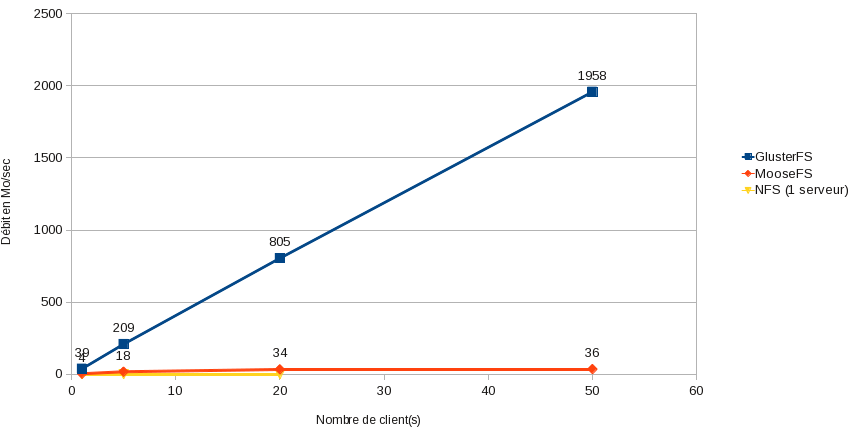
\includegraphics[width=1\linewidth]{graph/calc/50WS.png}
				        \caption{Écriture de petits fichiers avec 50 serveurs}
			        \end{center}
		        \end{figure}
\begin{figure}[H]
\begin{center}
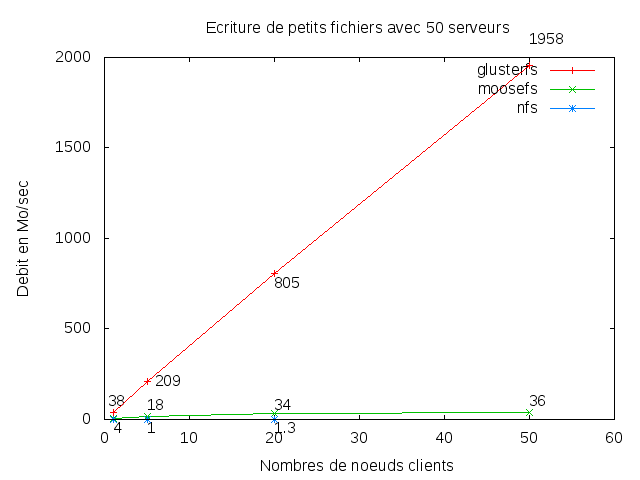
\includegraphics[bb=0 0 640 480,width=14cm]{images/srv50ws.png}
\caption{Écriture de petits fichiers avec 50 serveurs}
\end{center}
\end{figure} 
\begin{figure}[H]
\begin{center}
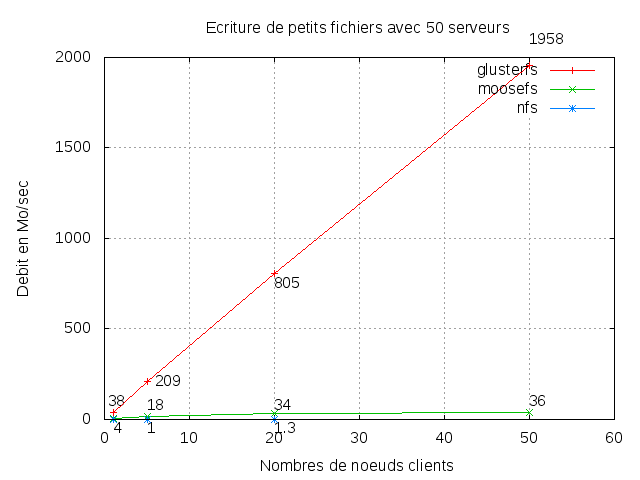
\includegraphics[bb=0 0 640 480,width=14cm]{images/srv50ws2.png}
\caption{Écriture de petits fichiers avec 50 serveurs}
\end{center}
\end{figure} 
		        \begin{figure}[H]
			        \begin{center}
				        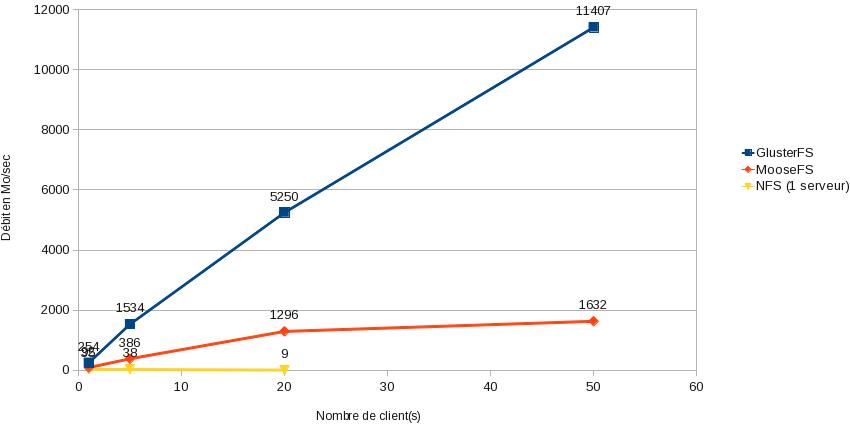
\includegraphics[width=1\linewidth]{graph/calc/50WB.png}
				        \caption{Écriture de gros fichiers avec 50 serveurs}
			        \end{center}
		        \end{figure}
\begin{figure}[H]
\begin{center}
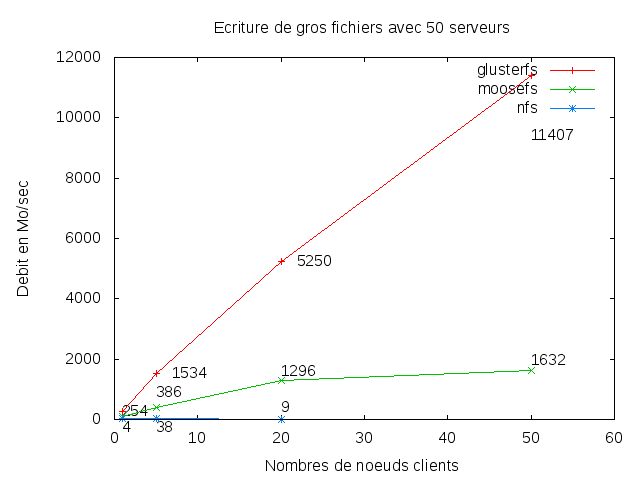
\includegraphics[bb=0 0 640 480,width=14cm]{images/srv50wb.png}
\caption{Écriture de gros fichiers avec 50 serveurs}
\end{center}
\end{figure} 
\begin{figure}[H]
\begin{center}
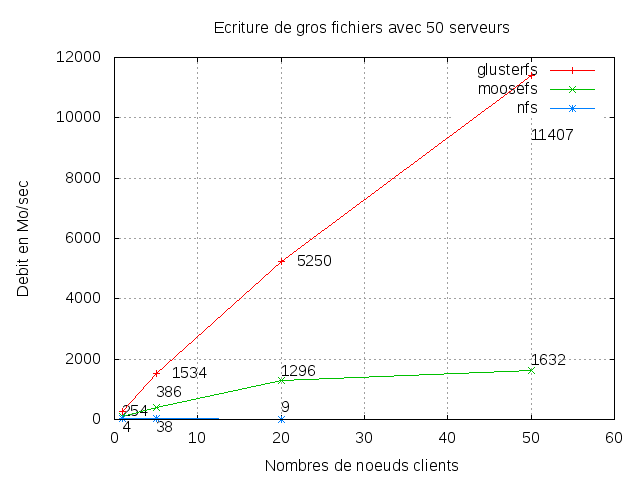
\includegraphics[bb=0 0 640 480,width=14cm]{images/srv50wb2.png}
\caption{Écriture de gros fichiers avec 50 serveurs}
\end{center}
\end{figure} 
		        \begin{figure}[H]
			        \begin{center}
				        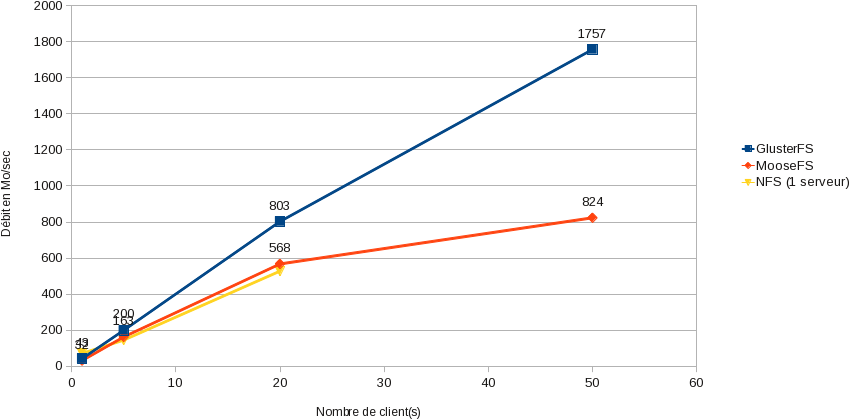
\includegraphics[width=1\linewidth]{graph/calc/50RS.png}
				        \caption{Lecture de petits fichiers avec 50 serveurs}
			        \end{center}
		        \end{figure}
\begin{figure}[H]
\begin{center}
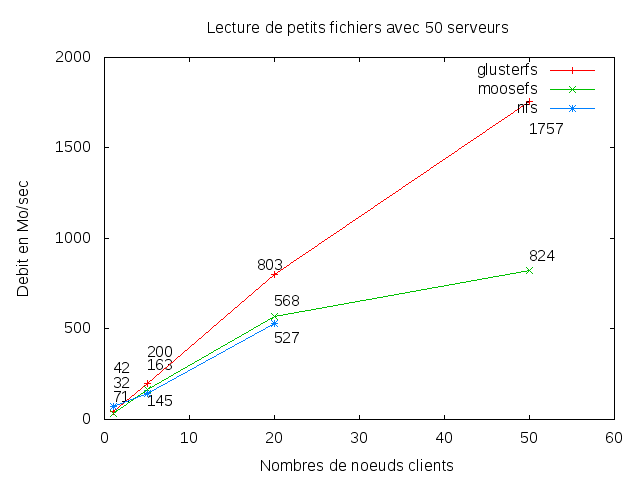
\includegraphics[bb=0 0 640 480,width=14cm]{images/srv50rs.png}
\caption{Écriture de gros fichiers avec 50 serveurs}
\end{center}
\end{figure} 
\begin{figure}[H]
\begin{center}
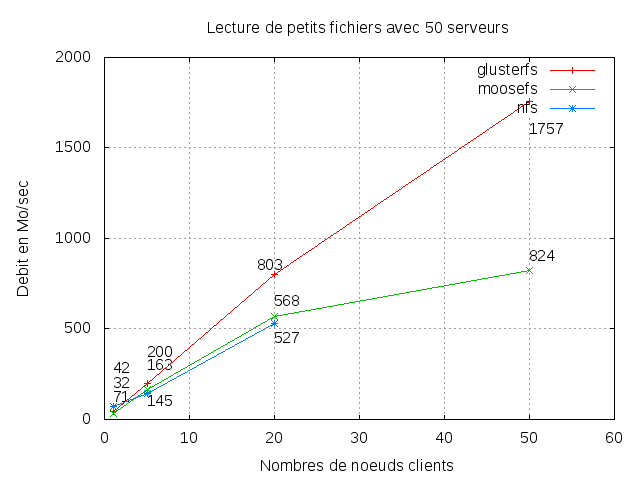
\includegraphics[bb=0 0 640 480,width=14cm]{images/srv50rs2.png}
\caption{Écriture de gros fichiers avec 50 serveurs}
\end{center}
\end{figure} 
		        \begin{figure}[H]
			        \begin{center}
				        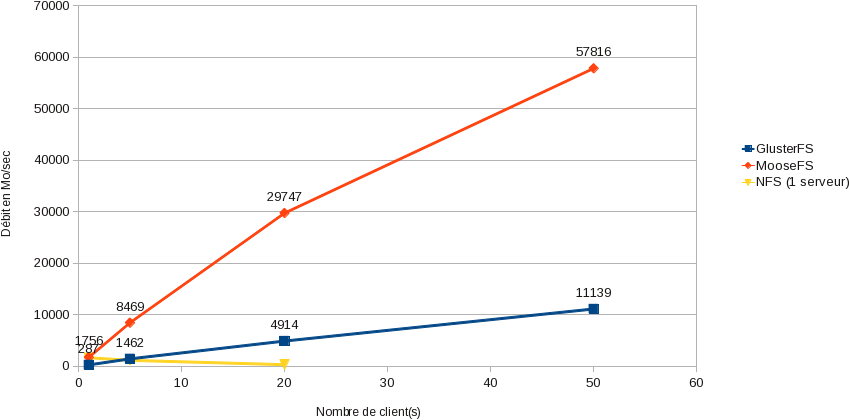
\includegraphics[width=1\linewidth]{graph/calc/50RB.png}
				        \caption{Lecture de gros fichiers avec 50 serveurs}
			        \end{center}
		        \end{figure}
\begin{figure}[H]
\begin{center}
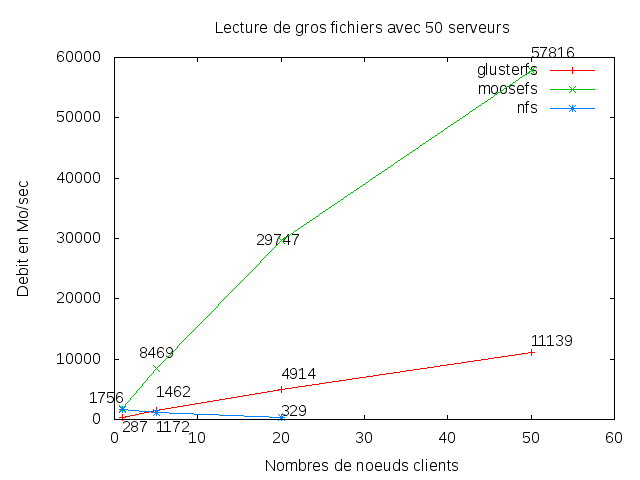
\includegraphics[bb=0 0 640 480,width=14cm]{images/srv50rb.png}
\caption{Écriture de gros fichiers avec 50 serveurs}
\end{center}
\end{figure} 
\begin{figure}[H]
\begin{center}
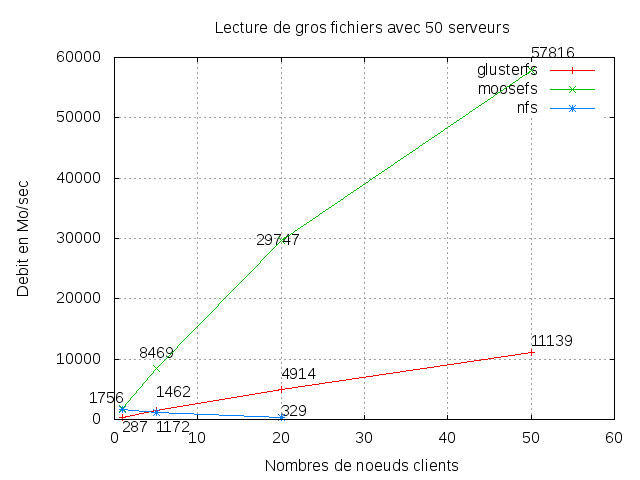
\includegraphics[bb=0 0 640 480,width=14cm]{images/srv50rb2.png}
\caption{Écriture de gros fichiers avec 50 serveurs}
\end{center}
\end{figure} 
			\subsection{Analyse des résultats}

			Sur les tests que nous avons effectués, nous remarquons des débits très importants, parfois supérieurs au débit du réseau présent sur le cluster.
			Nous nous sommes donc questionné, afin de trouver pourquoi nous obtenons de tels résultats, et nous avons émis les hypothèses suivantes :
			\begin{itemize}
				\item Lors de la lecture de fichiers (petits ou gros), le client lit des fichiers font il possède une copie sur sa machine,
				le systèmes de fichier distribué est-il capable de le détecter, et d'éviter d'aller lire le fichier sur un serveur distant ?
				\item Le cache présent sur les systèmes de fichiers est-il, à lui seul, responsable de tel résultats pour la lecture ?
				\item Lors des tests d'écriture, tous les clients écrivent les mêmes fichiers, le système de fichier distribué est-il capable de le détecter,
				et de limiter les transferts des clients vers les serveurs ?
			\end{itemize}

	\chapter{Conclusion}
	% sur les FS
	% sur nos objectifs de départ
	% apport du projet tuteuré pour nous, bonne expérience avant départ en stage, ...

	Durant ce projet tuteuré nous avons eut la chance de travailler sur une grande structure : le Grid'5000.
	Après un premier temps de prise en main, nous avons pu commencer à mettre en place des solutions de systèmes de fichiers distribués,
	à créer des scripts automatisant leurs déploiements, et à un réaliser un benchmark.\\

	Nous avons rencontré un certains nombre de difficultés, (en plus de la mise en place des systèmes de fichiers distribués) propre au Grid'5000 :
	\begin{itemize}
		\item Nos test devaient être réalisés sur un même cluster, mais nous n'étions pas seuls à travailler dessus,
		et on nous ne disposions pas toujours de toutes les machines dont nous avions besoins
		\item Nous avons aussi rencontré des erreurs lors de déploiement de machines, indépendant de nous, qui ont \og cassé\fg~ des benchmarks programmés à l'avance.
		\item Et nous avons aussi commis quelques erreurs humaines :
		\begin{itemize}
			\item Suppression d'une réservation \og importante\fg~ lors du nettoyage de l'espace de travail.
			\item Oubli de donner les droits d'exécution à un script de pilotage, lors d'une réservation \og importante\fg.\\
		\end{itemize}
	\end{itemize}

	A cause de ces divers problèmes, nous n'avons pas obtenus tous les résultats que nous avions prévus d'avoir, ce qui ne permet pas une comparaison aussi approfondi
	que nous avions souhaité.\\

	Le script de benchmark s'est aussi montré, après coup, imparfait, du fait que les clients lisent un fichier distant, dont ils ont une copie sur leurs machines,
	ce qui a pu fausser nos résultats.\\

	Malgré ces problèmes, nous avons quand même pu effectuer une comparaison de différents systèmes de fichiers distribués.
	Ce travail nous a offert une bonne expérience pratique, d'un sujet technique, avant notre départ en stage.

	\appendix
		\chapter{Organisation du travail}
			\section{Outils utilisés}
				Afin d'organiser au mieux notre travail, nous avons mise en place un projet sur GitHub
				\footnote{GitHub est un service web d'hébergement et de gestion de développement de logiciels (Wikipédia).}.
				Nous avons utilisé le wiki
				\footnote{Un wiki est un site Web dont les pages comportent des hyperliens les unes vers les autres
				et sont modifiables par les visiteurs afin de permettre l'écriture et l'illustration collaboratives des documents numériques qu'il contient. (Wikipédia)}
				mise à notre disposition afin de mettre en commun nos connaissances et nos découvertes sur notre projet.

				Nous avons aussi utilisé le dépôt Git\footnote{Git est un logiciel de gestion de versions, écrit par Linus Torvalds.} pour gérer le développement
				de nos scripts, et notre rapport de projet.
\newpage
			\section{Répartition des taches}
				\subsection{Florent Lévigne}
					\begin{itemize}
						\item Étude sur la mise en place de GlusterFS
						\item Réalisation d'un script de déploiement de GlusterFS
						\item Étude sur la mise en place de MooseFS
						\item Réalisation d'un script de déploiement de MooseFS
						\item Réalisation d'un script de benchmark pour système de fichiers distribué
						\item Rédaction du rapport
					\end{itemize}
				\subsection{Jean-François Garcia}
					\begin{itemize}
						\item Étude sur la mise en place de GlusterFS
						\item Étude sur la mise en place de NFS
						\item Réalisation d'un script de déploiement de NFS
						\item Étude sur la mise en place de CephFS
						\item Réalisation d'un script de déploiement de CephFS
					\end{itemize}
				\subsection{Maxime Douhéret}
					\begin{itemize}
						\item Étude sur la mise en place de GlusterFS
						\item Étude sur la mise en place de CephFS
						\item Aide à la réalisation des scripts de déploiement de CephFS et de benchmark
					\end{itemize}
				\subsection{Vincent Claudel}
					\begin{itemize}
						\item Étude sur la mise en place de GlusterFS
						\item Étude sur la mise en place de MooseFS
						\item Rédaction du rapport
						\item Réalisation des graphiques en GnuPlot
					\end{itemize}	
		\chapter{Scripts}
			\section{GlusterFS}
				Fichier deploimentGluster.rb :
				\lstinputlisting[language=Ruby,numbers=left]{../glusterFs/deploiementGluster.rb}
				% autre fichier (améliorer le script)
			\section{MooseFs}
                                Fichier deploiementMoose.rb :
                                \lstinputlisting[language=Ruby,numbers=left]{../mooseFs/deploiementMoose.rb}
                                Fichier masterServer.sh :
                                \lstinputlisting[language=Ruby,numbers=left]{../mooseFs/masterServer.sh}
\newpage
                                Fichier chunkServer.rb :
                                \lstinputlisting[language=Ruby,numbers=left]{../mooseFs/chunkServer.rb}
                                Fichier metaloggerServer.sh :
                                \lstinputlisting[language=Ruby,numbers=left]{../mooseFs/metaloggerServer.sh}
                                Fichier client.sh :
                                \lstinputlisting[language=Ruby,numbers=left]{../mooseFs/client.sh}
			\section{Ceph}
				Fichier deploimentCeph.rb :
				\lstinputlisting[language=Ruby,numbers=left]{../cephFS/deploiementCeph.rb}
			\section{NFS}
				Fichier deploimentNFS.rb :
				\lstinputlisting[language=Ruby,numbers=left]{../NFS/deploiementNFS.rb}
			\section{Benchmark}
				Fichier benchmark.rb :
				\lstinputlisting[language=Ruby,numbers=left]{../benchmark/benchmark.rb}

				Fichier writingSmallFiles.sh :
				\lstinputlisting[language=Bash,numbers=left]{../benchmark/writingSmallFiles.sh}

				Fichier writingBigFiles.sh :
				\lstinputlisting[language=Bash,numbers=left]{../benchmark/writingBigFiles.sh}

				Fichier readingSmallFiles.sh :
				\lstinputlisting[language=Bash,numbers=left]{../benchmark/readingSmallFiles.sh}

				Fichier readingBigFile.sh :
				\lstinputlisting[language=Bash, numbers=left]{../benchmark/readingBigFile.sh}
			\section{Meta scripts}
				Fichier meta\_NFS.sh :
				\lstinputlisting[language=Bash,numbers=left]{../metascript/meta_NFS.sh}

				Fichier meta\_gluster.sh :
				\lstinputlisting[language=Bash,numbers=left]{../metascript/meta_gluster.sh}

				Fichier meta\_ceph.sh :
				\lstinputlisting[language=Bash,numbers=left]{../metascript/meta_ceph.sh}

				Fichier meta\_moose.sh :
				\lstinputlisting[language=Bash,numbers=left]{../metascript/meta_moose.sh}

		\chapter{Résultats relevés}

			\section{NFS}

			Écriture de petits fichiers avec NFS (débit en Mo/sec) :

			\begin{tabular}{|l|c|c|c|c|}
				\hline
				& 1 client & 5 clients & 20 clients & 50 clients \\
				\hline
				1 serveur & 1.76 & 1.17 & 1.31 & \\
				\hline
			\end{tabular}\\\\

			Écriture de gros fichiers avec NFS (débit en Mo/sec) :

			\begin{tabular}{|l|c|c|c|c|}
				\hline
				& 1 client & 5 clients & 20 clients & 50 clients \\
				\hline
				1 serveur & 35.11 & 37.83 & 8.54 & \\
				\hline
			\end{tabular}\\\\

			Lecture de petits fichiers avec NFS (débit en Mo/sec) :

			\begin{tabular}{|l|c|c|c|c|}
				\hline
				& 1 client & 5 clients & 20 clients & 50 clients \\
				\hline
				 1 serveur & 71.53 & 145.78 & 527.97 & \\
				\hline
			\end{tabular}\\\\

			Lecture de gros fichiers avec NFS (débit en Mo/sec) :

			\begin{tabular}{|l|c|c|c|c|}
				\hline
				& 1 client & 5 clients & 20 clients & 50 clients \\
				\hline
				1 serveur & 1675.29 & 1172.55 & 329.87& \\
				\hline
			\end{tabular}

			\newpage

			\section{GlusterFS}

			Écriture de petits fichiers avec GlusterFS (débit en Mo/sec) :

			\begin{tabular}{|l|c|c|c|c|}
				\hline
				& 1 client & 5 clients & 20 clients & 50 clients \\
				\hline
				5 serveurs & & & & \\
				\hline
				20 serveurs & & & & \\
				\hline
				50 serveurs & 38.55 & 209.48 & 804.68 & 1957.51 \\
				\hline
			\end{tabular}\\\\

			Écriture de gros fichiers avec GlusterFS (débit en Mo/sec) :

			\begin{tabular}{|l|c|c|c|c|}
				\hline
				& 1 client & 5 clients & 20 clients & 50 clients \\
				\hline
				5 serveurs & & & & \\
				\hline
				20 serveurs & & & & \\
				\hline
				50 serveurs & 254.01 & 1533.95 & 5249.86 & 11407.30 \\
				\hline
			\end{tabular}\\\\

			Lecture de petits fichiers avec GlusterFS (débit en Mo/sec) :

			\begin{tabular}{|l|c|c|c|c|}
				\hline
				& 1 client & 5 clients & 20 clients & 50 clients \\
				\hline
				5 serveurs & & & & \\
				\hline
				20 serveurs & & & & \\
				\hline
				50 serveurs & 42.82 & 200.15 & 802.95 & 1756.84 \\
				\hline
			\end{tabular}\\\\

			Lecture de gros fichiers avec GlusterFS (débit en Mo/sec) :

			\begin{tabular}{|l|c|c|c|c|}
				\hline
				& 1 client & 5 clients & 20 clients & 50 clients \\
				\hline
				5 serveurs & & & & \\
				\hline
				20 serveurs & & & & \\
				\hline
				50 serveurs & 287.22 & 1461.58 & 4914.09 & 11139.07 \\
				\hline
			\end{tabular}

			\newpage

			\section{MooseFS}

			\textbf{Les résultats de MooseFS avec 5 serveurs ont été obtenus sur un autre cluster.}\\

			Écriture de petits fichiers avec MooseFS (débit en Mo/sec) :

			\begin{tabular}{|l|c|c|c|c|}
				\hline
				& 1 client & 5 clients & 20 clients & 50 clients \\
				\hline
				5 serveurs & 2.43 & 5.58 & 15.14 & 14.53 \\
				\hline
				20 serveurs & 4.37 & 13.93 & 17.93 & 17.80 \\
				\hline
				50 serveurs & 4.17 & 18.01 & 34.35 & 36.22 \\
				\hline
			\end{tabular}\\\\

			Écriture de gros fichiers avec MooseFS (débit en Mo/sec) :

			\begin{tabular}{|l|c|c|c|c|}
				\hline
				& 1 client & 5 clients & 20 clients & 50 clients \\
				\hline
				5 serveurs & 21554.35 & 2536.51 & 9901.15 & 23020.77 \\
				\hline
				20 serveurs & 79.83 & 308.10 & 573.01 & 545.86 \\
				\hline
				50 serveurs & 92.33 & 385.99 & 1295.74 & 1631.78 \\
				\hline
			\end{tabular}\\\\

			Lecture de petits fichiers avec MooseFS (débit en Mo/sec) :

			\begin{tabular}{|l|c|c|c|c|}
				\hline
				& 1 client & 5 clients & 20 clients & 50 clients \\
				\hline
				5 serveurs & 31.54 & 162.36 & 667.75 & 1485.40 \\
				\hline
				20 serveurs & 35.03 & 172.10 & 569.37 & 853.36 \\
				\hline
				50 serveurs & 31.97 & 163.32 & 567.77 & 823.54 \\
				\hline
			\end{tabular}\\\\

			Lecture de gros fichiers avec MooseFS (débit en Mo/sec) :

			\begin{tabular}{|l|c|c|c|c|}
				\hline
				& 1 client & 5 clients & 20 clients & 50 clients \\
				\hline
				5 serveurs & 21093.63 & 2540.53 & 9928.70 & 23112.12 \\
				\hline
				20 serveurs & 1779.99 & 8525.03 & 31322.11 & 64509.88 \\
				\hline
				50 serveurs & 1755.61 & 8468.74 & 29746.91 & 57816.35 \\
				\hline
			\end{tabular}

			\newpage

			\section{Ceph}

			\textbf{Les résultats de Ceph avec 5 serveurs ont été obtenus sur un autre cluster.}\\

			Écriture de petits fichiers avec Ceph (débit en Mo/sec) :

			\begin{tabular}{|l|c|c|c|c|}
				\hline
				& 1 client & 5 clients & 20 clients & 50 clients \\
				\hline
				5 serveurs & 6.02 & 6.06 & 27.12 & 31.04 \\
				\hline
				20 serveurs & & & & \\
				\hline
				50 serveurs & & & & \\
				\hline
			\end{tabular}\\\\

			Écriture de gros fichiers avec Ceph (débit en Mo/sec) :

			\begin{tabular}{|l|c|c|c|c|}
				\hline
				& 1 client & 5 clients & 20 clients & 50 clients \\
				\hline
				5 serveurs & 6.02 & 6.06 & 6.20 & 6.47 \\
				\hline
				20 serveurs & & & & \\
				\hline
				50 serveurs & & & & \\
				\hline
			\end{tabular}\\\\

			Lecture de petits fichiers avec Ceph (débit en Mo/sec) :

			\begin{tabular}{|l|c|c|c|c|}
				\hline
				& 1 client & 5 clients & 20 clients & 50 clients \\
				\hline
				5 serveurs & 6.01 & 6.06 & 6.20 & 6.48 \\
				\hline
				20 serveurs & & & & \\
				\hline
				50 serveurs & & & & \\
				\hline
			\end{tabular}\\\\

			Lecture de gros fichiers avec Ceph (débit en Mo/sec) :

			\begin{tabular}{|l|c|c|c|c|}
				\hline
				& 1 client & 5 clients & 20 clients & 50 clients \\
				\hline
				5 serveurs & 6.02 & 6.06 & 6.20 & 6.47 \\
				\hline
				20 serveurs & & & & \\
				\hline
				50 serveurs & & & & \\
				\hline
			\end{tabular}

		\chapter{Sources}

			\begin{itemize}
				\item Pour l'ensemble de notre travail : Wikipédia Français et Anglais
				\item NFS :
				\item GlusterFS :
				\begin{itemize}
					\item Documentation de GlusterFS\footnote{\href{http://gluster.com/community/documentation/index.php/Main_Page}
					{http://gluster.com/community/documentation/index.php/Main\_Page}}
					\item Gnu/Linux Magazine numéro 133 : \og Introduction à GlusterFS\fg
				\end{itemize}
				\item MooseFS :
				\begin{itemize}
					\item Documentation de MooseFS\footnote{\href{http://www.moosefs.org/reference-guide.html}{http://www.moosefs.org/reference-guide.html}}, en particulier
					\og Installing MooseFS Step by Step Tutorial\fg
					\footnote{\href{http://www.moosefs.org/tl_files/manpageszip/moosefs-step-by-step-tutorial-v.1.1.pdf}
					{http://www.moosefs.org/tl\_files/manpageszip/moosefs-step-by-step-tutorial-v.1.1.pdf}}
				\end{itemize}
				\item Ceph :
			\end{itemize}

\end{document}

